% Options for packages loaded elsewhere
\PassOptionsToPackage{unicode}{hyperref}
\PassOptionsToPackage{hyphens}{url}
%
\documentclass[
]{book}
\usepackage{amsmath,amssymb}
\usepackage{iftex}
\ifPDFTeX
  \usepackage[T1]{fontenc}
  \usepackage[utf8]{inputenc}
  \usepackage{textcomp} % provide euro and other symbols
\else % if luatex or xetex
  \usepackage{unicode-math} % this also loads fontspec
  \defaultfontfeatures{Scale=MatchLowercase}
  \defaultfontfeatures[\rmfamily]{Ligatures=TeX,Scale=1}
\fi
\usepackage{lmodern}
\ifPDFTeX\else
  % xetex/luatex font selection
\fi
% Use upquote if available, for straight quotes in verbatim environments
\IfFileExists{upquote.sty}{\usepackage{upquote}}{}
\IfFileExists{microtype.sty}{% use microtype if available
  \usepackage[]{microtype}
  \UseMicrotypeSet[protrusion]{basicmath} % disable protrusion for tt fonts
}{}
\makeatletter
\@ifundefined{KOMAClassName}{% if non-KOMA class
  \IfFileExists{parskip.sty}{%
    \usepackage{parskip}
  }{% else
    \setlength{\parindent}{0pt}
    \setlength{\parskip}{6pt plus 2pt minus 1pt}}
}{% if KOMA class
  \KOMAoptions{parskip=half}}
\makeatother
\usepackage{xcolor}
\usepackage{color}
\usepackage{fancyvrb}
\newcommand{\VerbBar}{|}
\newcommand{\VERB}{\Verb[commandchars=\\\{\}]}
\DefineVerbatimEnvironment{Highlighting}{Verbatim}{commandchars=\\\{\}}
% Add ',fontsize=\small' for more characters per line
\usepackage{framed}
\definecolor{shadecolor}{RGB}{248,248,248}
\newenvironment{Shaded}{\begin{snugshade}}{\end{snugshade}}
\newcommand{\AlertTok}[1]{\textcolor[rgb]{0.94,0.16,0.16}{#1}}
\newcommand{\AnnotationTok}[1]{\textcolor[rgb]{0.56,0.35,0.01}{\textbf{\textit{#1}}}}
\newcommand{\AttributeTok}[1]{\textcolor[rgb]{0.13,0.29,0.53}{#1}}
\newcommand{\BaseNTok}[1]{\textcolor[rgb]{0.00,0.00,0.81}{#1}}
\newcommand{\BuiltInTok}[1]{#1}
\newcommand{\CharTok}[1]{\textcolor[rgb]{0.31,0.60,0.02}{#1}}
\newcommand{\CommentTok}[1]{\textcolor[rgb]{0.56,0.35,0.01}{\textit{#1}}}
\newcommand{\CommentVarTok}[1]{\textcolor[rgb]{0.56,0.35,0.01}{\textbf{\textit{#1}}}}
\newcommand{\ConstantTok}[1]{\textcolor[rgb]{0.56,0.35,0.01}{#1}}
\newcommand{\ControlFlowTok}[1]{\textcolor[rgb]{0.13,0.29,0.53}{\textbf{#1}}}
\newcommand{\DataTypeTok}[1]{\textcolor[rgb]{0.13,0.29,0.53}{#1}}
\newcommand{\DecValTok}[1]{\textcolor[rgb]{0.00,0.00,0.81}{#1}}
\newcommand{\DocumentationTok}[1]{\textcolor[rgb]{0.56,0.35,0.01}{\textbf{\textit{#1}}}}
\newcommand{\ErrorTok}[1]{\textcolor[rgb]{0.64,0.00,0.00}{\textbf{#1}}}
\newcommand{\ExtensionTok}[1]{#1}
\newcommand{\FloatTok}[1]{\textcolor[rgb]{0.00,0.00,0.81}{#1}}
\newcommand{\FunctionTok}[1]{\textcolor[rgb]{0.13,0.29,0.53}{\textbf{#1}}}
\newcommand{\ImportTok}[1]{#1}
\newcommand{\InformationTok}[1]{\textcolor[rgb]{0.56,0.35,0.01}{\textbf{\textit{#1}}}}
\newcommand{\KeywordTok}[1]{\textcolor[rgb]{0.13,0.29,0.53}{\textbf{#1}}}
\newcommand{\NormalTok}[1]{#1}
\newcommand{\OperatorTok}[1]{\textcolor[rgb]{0.81,0.36,0.00}{\textbf{#1}}}
\newcommand{\OtherTok}[1]{\textcolor[rgb]{0.56,0.35,0.01}{#1}}
\newcommand{\PreprocessorTok}[1]{\textcolor[rgb]{0.56,0.35,0.01}{\textit{#1}}}
\newcommand{\RegionMarkerTok}[1]{#1}
\newcommand{\SpecialCharTok}[1]{\textcolor[rgb]{0.81,0.36,0.00}{\textbf{#1}}}
\newcommand{\SpecialStringTok}[1]{\textcolor[rgb]{0.31,0.60,0.02}{#1}}
\newcommand{\StringTok}[1]{\textcolor[rgb]{0.31,0.60,0.02}{#1}}
\newcommand{\VariableTok}[1]{\textcolor[rgb]{0.00,0.00,0.00}{#1}}
\newcommand{\VerbatimStringTok}[1]{\textcolor[rgb]{0.31,0.60,0.02}{#1}}
\newcommand{\WarningTok}[1]{\textcolor[rgb]{0.56,0.35,0.01}{\textbf{\textit{#1}}}}
\usepackage{longtable,booktabs,array}
\usepackage{calc} % for calculating minipage widths
% Correct order of tables after \paragraph or \subparagraph
\usepackage{etoolbox}
\makeatletter
\patchcmd\longtable{\par}{\if@noskipsec\mbox{}\fi\par}{}{}
\makeatother
% Allow footnotes in longtable head/foot
\IfFileExists{footnotehyper.sty}{\usepackage{footnotehyper}}{\usepackage{footnote}}
\makesavenoteenv{longtable}
\usepackage{graphicx}
\makeatletter
\def\maxwidth{\ifdim\Gin@nat@width>\linewidth\linewidth\else\Gin@nat@width\fi}
\def\maxheight{\ifdim\Gin@nat@height>\textheight\textheight\else\Gin@nat@height\fi}
\makeatother
% Scale images if necessary, so that they will not overflow the page
% margins by default, and it is still possible to overwrite the defaults
% using explicit options in \includegraphics[width, height, ...]{}
\setkeys{Gin}{width=\maxwidth,height=\maxheight,keepaspectratio}
% Set default figure placement to htbp
\makeatletter
\def\fps@figure{htbp}
\makeatother
\setlength{\emergencystretch}{3em} % prevent overfull lines
\providecommand{\tightlist}{%
  \setlength{\itemsep}{0pt}\setlength{\parskip}{0pt}}
\setcounter{secnumdepth}{5}
\usepackage{booktabs}
\usepackage{booktabs}
\usepackage{longtable}
\usepackage{array}
\usepackage{multirow}
\usepackage{wrapfig}
\usepackage{float}
\usepackage{colortbl}
\usepackage{pdflscape}
\usepackage{tabularx}
\usepackage{xltabular}
\usepackage{threeparttable}
\usepackage{threeparttablex}
\usepackage[normalem]{ulem}
\usepackage{makecell}
\usepackage{xcolor}
\ifLuaTeX
  \usepackage{selnolig}  % disable illegal ligatures
\fi
\usepackage[]{natbib}
\bibliographystyle{plainnat}
\usepackage{bookmark}
\IfFileExists{xurl.sty}{\usepackage{xurl}}{} % add URL line breaks if available
\urlstyle{same}
\hypersetup{
  pdfauthor={Veronique Voisin},
  hidelinks,
  pdfcreator={LaTeX via pandoc}}

\title{
\includegraphics[width=\textwidth,height=1.04167in]{image/CBW_logo.png}

Cancer Workshop 2026 - Module 8: Pathway Enrichment Analysis}
\author{Veronique Voisin}
\date{October 2026}

\begin{document}
\maketitle

{
\setcounter{tocdepth}{1}
\tableofcontents
}
\textbf{This work is licensed under a \href{https://creativecommons.org/licenses/by-sa/4.0/deed.en}{Creative Commons Attribution-ShareAlike 4.0 Unported License}. This means that you are able to copy, share and modify the work, as long as the result is distributed under the same license.}

This module will cover how to use differential expression output to generate pathway enrichment results.

\chapter*{Presentation of the dataset}\label{presentation-of-the-dataset}
\addcontentsline{toc}{chapter}{Presentation of the dataset}

\begin{itemize}
\item
  This module is a continuation of the transcriptomics module 6 and we will use the same dataset. This dataset contains bulk RNA-seq data of a model of breast cancer. The gene counts were deposited to the Gene Expression Omnibus (GEO) database under accession \textbf{\emph{GSE222367}} and are publicly available.
\item
  RNA was extracted from MCF7, a breast cancer cell line under different conditions: parental cell line and cell line samples resistant to the drugs palbociclib or abemaciclib.
\item
  Biological replicates were available for each condition.
\item
  RNA-seq library was prepared and sequenced using an Illumina HiSeq 2500 sequencer.
\item
  Sequence reads were mapped to the human reference genome (Gencode GRCh38) using TopHat as aligner.
\item
  The BAM files with mapped reads for each sample were sorted and then used as input for HTSeq 0.11.0 in order to generate read count data at the gene level.
\item
  We retrieved the gene counts and performed differential expression analysis using a negative binomial generalized linear model, followed by pathway enrichment analysis.
\end{itemize}

\begin{figure}
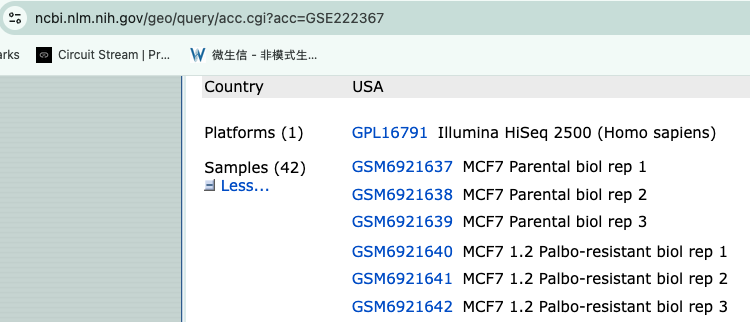
\includegraphics[width=0.6\linewidth]{image/GEOscreenshot} \caption{GEO dataset}\label{fig:fig-mychart}
\end{figure}

\chapter*{Differential Expression}\label{differential-expression}
\addcontentsline{toc}{chapter}{Differential Expression}

\textbf{This work is licensed under a \href{https://creativecommons.org/licenses/by-sa/4.0/deed.en}{Creative Commons Attribution-ShareAlike 4.0 Unported License}. This means that you are able to copy, share and modify the work, as long as the result is distributed under the same license.}

We perform differential expression analysis using a negative binomial generalized linear model using the edgeR package.

\section{Install and load libraries}\label{install-and-load-libraries}

\begin{Shaded}
\begin{Highlighting}[]
\DocumentationTok{\#\# CRAN and Bioconductor setup}
\ControlFlowTok{if}\NormalTok{ (}\SpecialCharTok{!}\FunctionTok{requireNamespace}\NormalTok{(}\StringTok{"BiocManager"}\NormalTok{, }\AttributeTok{quietly =} \ConstantTok{TRUE}\NormalTok{))}
  \FunctionTok{install.packages}\NormalTok{(}\StringTok{"BiocManager"}\NormalTok{)}

\DocumentationTok{\#\# List of CRAN packages}
\NormalTok{cran\_packages }\OtherTok{\textless{}{-}} \FunctionTok{c}\NormalTok{(}
  \StringTok{"tidyverse"}\NormalTok{,}
  \StringTok{"gprofiler2"}\NormalTok{,}
  \StringTok{"ggrepel"}
\NormalTok{)}

\CommentTok{\# List of Bioconductor packages}
\NormalTok{bioc\_packages }\OtherTok{\textless{}{-}} \FunctionTok{c}\NormalTok{(}
  \StringTok{"edgeR"}\NormalTok{,}
  \StringTok{"fgsea"}
\NormalTok{)}

\CommentTok{\# Install CRAN packages if not already installed}
\ControlFlowTok{for}\NormalTok{ (pkg }\ControlFlowTok{in}\NormalTok{ cran\_packages) \{}
  \ControlFlowTok{if}\NormalTok{ (}\SpecialCharTok{!}\FunctionTok{requireNamespace}\NormalTok{(pkg, }\AttributeTok{quietly =} \ConstantTok{TRUE}\NormalTok{)) \{}
    \FunctionTok{install.packages}\NormalTok{(pkg)}
\NormalTok{  \}}
\NormalTok{\}}

\CommentTok{\# Install Bioconductor packages if not already installed}
\ControlFlowTok{for}\NormalTok{ (pkg }\ControlFlowTok{in}\NormalTok{ bioc\_packages) \{}
  \ControlFlowTok{if}\NormalTok{ (}\SpecialCharTok{!}\FunctionTok{requireNamespace}\NormalTok{(pkg, }\AttributeTok{quietly =} \ConstantTok{TRUE}\NormalTok{)) \{}
\NormalTok{    BiocManager}\SpecialCharTok{::}\FunctionTok{install}\NormalTok{(pkg)}
\NormalTok{  \}}
\NormalTok{\}}

\CommentTok{\# Load the libraries}

\CommentTok{\# CRAN packages}
\FunctionTok{library}\NormalTok{(tidyverse)}
\end{Highlighting}
\end{Shaded}

\begin{verbatim}
## -- Attaching core tidyverse packages ------------------------ tidyverse 2.0.0 --
## v dplyr     1.2.1     v readr     2.2.0
## v forcats   1.0.1     v stringr   1.6.0
## v ggplot2   4.0.3     v tibble    3.3.1
## v lubridate 1.9.5     v tidyr     1.3.2
## v purrr     1.2.2     
## -- Conflicts ------------------------------------------ tidyverse_conflicts() --
## x dplyr::filter() masks stats::filter()
## x dplyr::lag()    masks stats::lag()
## i Use the conflicted package (<http://conflicted.r-lib.org/>) to force all conflicts to become errors
\end{verbatim}

\begin{Shaded}
\begin{Highlighting}[]
\FunctionTok{library}\NormalTok{(gprofiler2)}
\FunctionTok{library}\NormalTok{(ggrepel)}
\CommentTok{\# Bioconductor packages}
\FunctionTok{library}\NormalTok{(edgeR)}
\end{Highlighting}
\end{Shaded}

\begin{verbatim}
## Loading required package: limma
\end{verbatim}

\begin{Shaded}
\begin{Highlighting}[]
\FunctionTok{library}\NormalTok{(fgsea)}
\end{Highlighting}
\end{Shaded}

\section{Data used for this comparison}\label{data-used-for-this-comparison}

For this analysis, we are going to compare the Palbo-resistant cell lines (3 biological replicates) versus the parental cell lines (3 biological replicates)

\begin{figure}
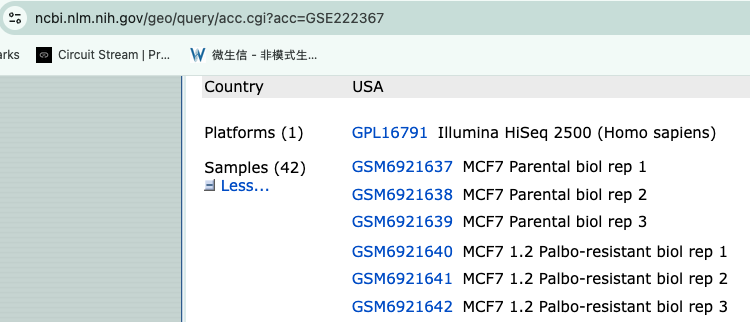
\includegraphics[width=0.6\linewidth]{image/GEOscreenshot} \caption{GEO dataset}\label{fig:dataset}
\end{figure}

\subsection{generate a DGE object}\label{generate-a-dge-object}

\begin{Shaded}
\begin{Highlighting}[]
\CommentTok{\# 1. Find the count files}
\NormalTok{files }\OtherTok{\textless{}{-}} \FunctionTok{list.files}\NormalTok{(}\AttributeTok{path =} \StringTok{"data"}\NormalTok{, }\AttributeTok{pattern =} \StringTok{"}\SpecialCharTok{\textbackslash{}\textbackslash{}}\StringTok{.txt}\SpecialCharTok{\textbackslash{}\textbackslash{}}\StringTok{.gz$"}\NormalTok{, }\AttributeTok{full.names =} \ConstantTok{TRUE}\NormalTok{)}

\CommentTok{\# 2. Sample names from the file names (strip the extension)}
\NormalTok{samples }\OtherTok{\textless{}{-}} \FunctionTok{sub}\NormalTok{(}\StringTok{"\_S.*"}\NormalTok{, }\StringTok{""}\NormalTok{, }\FunctionTok{basename}\NormalTok{(files))}

\CommentTok{\# 3. Read the files into a DGEList}
\CommentTok{\#    HTSeq output has no header: column 1 = gene ID, column 2 = count.}
\CommentTok{\#    R reads gzipped files directly, so no need to decompress.}
\NormalTok{dge }\OtherTok{\textless{}{-}} \FunctionTok{readDGE}\NormalTok{(files, }\AttributeTok{columns =} \FunctionTok{c}\NormalTok{(}\DecValTok{1}\NormalTok{, }\DecValTok{2}\NormalTok{), }\AttributeTok{header =} \ConstantTok{FALSE}\NormalTok{, }\AttributeTok{labels =}\NormalTok{ samples)}
\end{Highlighting}
\end{Shaded}

\begin{verbatim}
## Meta tags detected: __no_feature, __ambiguous, __too_low_aQual, __not_aligned, __alignment_not_unique
\end{verbatim}

\begin{Shaded}
\begin{Highlighting}[]
\CommentTok{\# 4. Remove HTSeq summary rows (\_\_no\_feature, \_\_ambiguous, etc.)}
\NormalTok{dge }\OtherTok{\textless{}{-}}\NormalTok{ dge[}\SpecialCharTok{!}\FunctionTok{grepl}\NormalTok{(}\StringTok{"\^{}\_\_"}\NormalTok{, }\FunctionTok{rownames}\NormalTok{(dge)), , keep.lib.sizes }\OtherTok{=} \ConstantTok{FALSE}\NormalTok{]}

\CommentTok{\# 5. (Optional) add group information}
\NormalTok{dge}\SpecialCharTok{$}\NormalTok{samples}\SpecialCharTok{$}\NormalTok{group }\OtherTok{\textless{}{-}} \FunctionTok{factor}\NormalTok{(}
  \FunctionTok{c}\NormalTok{(}\StringTok{"parental"}\NormalTok{, }\StringTok{"parental"}\NormalTok{, }\StringTok{"parental"}\NormalTok{,}
    \StringTok{"palbo\_resistant"}\NormalTok{, }\StringTok{"palbo\_resistant"}\NormalTok{, }\StringTok{"palbo\_resistant"}\NormalTok{),}
  \AttributeTok{levels =} \FunctionTok{c}\NormalTok{(}\StringTok{"parental"}\NormalTok{, }\StringTok{"palbo\_resistant"}\NormalTok{)   }\CommentTok{\# parental = reference}
\NormalTok{)}
\end{Highlighting}
\end{Shaded}

\section{Filter low-count genes and TMM-normalize}\label{filter-low-count-genes-and-tmm-normalize}

\begin{Shaded}
\begin{Highlighting}[]
\NormalTok{keep }\OtherTok{\textless{}{-}} \FunctionTok{filterByExpr}\NormalTok{(dge, }\AttributeTok{group =}\NormalTok{ dge}\SpecialCharTok{$}\NormalTok{samples}\SpecialCharTok{$}\NormalTok{group)}
\NormalTok{dge  }\OtherTok{\textless{}{-}}\NormalTok{ dge[keep, , keep.lib.sizes }\OtherTok{=} \ConstantTok{FALSE}\NormalTok{]}
\NormalTok{dge  }\OtherTok{\textless{}{-}} \FunctionTok{calcNormFactors}\NormalTok{(dge, }\AttributeTok{method =} \StringTok{"TMM"}\NormalTok{)}
\FunctionTok{cat}\NormalTok{(}\StringTok{"Genes retained after filtering:"}\NormalTok{, }\FunctionTok{nrow}\NormalTok{(dge), }\StringTok{"}\SpecialCharTok{\textbackslash{}n}\StringTok{"}\NormalTok{)}
\end{Highlighting}
\end{Shaded}

\begin{verbatim}
## Genes retained after filtering: 15246
\end{verbatim}

\begin{Shaded}
\begin{Highlighting}[]
\NormalTok{mds }\OtherTok{\textless{}{-}} \FunctionTok{plotMDS}\NormalTok{(dge, }\AttributeTok{col =} \FunctionTok{as.numeric}\NormalTok{(dge}\SpecialCharTok{$}\NormalTok{samples}\SpecialCharTok{$}\NormalTok{group), }\AttributeTok{main =} \StringTok{"MDS (logCPM)"}\NormalTok{)}
\end{Highlighting}
\end{Shaded}

\begin{Shaded}
\begin{Highlighting}[]
\NormalTok{group }\OtherTok{=}\NormalTok{ dge}\SpecialCharTok{$}\NormalTok{samples}\SpecialCharTok{$}\NormalTok{group}
\NormalTok{var\_pct }\OtherTok{\textless{}{-}} \FunctionTok{round}\NormalTok{(}\DecValTok{100} \SpecialCharTok{*}\NormalTok{ mds}\SpecialCharTok{$}\NormalTok{var.explained[mds}\SpecialCharTok{$}\NormalTok{dim.plot])}
\NormalTok{mds\_df }\OtherTok{\textless{}{-}} \FunctionTok{data.frame}\NormalTok{(}\AttributeTok{dim1 =}\NormalTok{ mds}\SpecialCharTok{$}\NormalTok{x, }\AttributeTok{dim2 =}\NormalTok{ mds}\SpecialCharTok{$}\NormalTok{y,}
                      \AttributeTok{sample =} \FunctionTok{colnames}\NormalTok{(dge), }\AttributeTok{group =}\NormalTok{ group)}

\FunctionTok{ggplot}\NormalTok{(mds\_df, }\FunctionTok{aes}\NormalTok{(}\AttributeTok{x =}\NormalTok{ dim1, }\AttributeTok{y =}\NormalTok{ dim2, }\AttributeTok{color =}\NormalTok{ group)) }\SpecialCharTok{+}
  \FunctionTok{geom\_point}\NormalTok{(}\AttributeTok{size =} \DecValTok{3}\NormalTok{) }\SpecialCharTok{+}
\NormalTok{  ggrepel}\SpecialCharTok{::}\FunctionTok{geom\_text\_repel}\NormalTok{(}\FunctionTok{aes}\NormalTok{(}\AttributeTok{label =}\NormalTok{ sample), }\AttributeTok{size =} \DecValTok{3}\NormalTok{, }\AttributeTok{color =} \StringTok{"grey30"}\NormalTok{,}
                            \AttributeTok{show.legend =} \ConstantTok{FALSE}\NormalTok{, }\AttributeTok{max.overlaps =} \ConstantTok{Inf}\NormalTok{,}
                            \AttributeTok{box.padding =} \FloatTok{0.4}\NormalTok{, }\AttributeTok{segment.color =} \StringTok{"grey60"}\NormalTok{) }\SpecialCharTok{+}
  \FunctionTok{labs}\NormalTok{(}\AttributeTok{title =} \StringTok{"MDS plot (all samples)"}\NormalTok{,}
       \AttributeTok{x =} \FunctionTok{sprintf}\NormalTok{(}\StringTok{"Leading logFC dim \%d (\%d\%\%)"}\NormalTok{, mds}\SpecialCharTok{$}\NormalTok{dim.plot[}\DecValTok{1}\NormalTok{], var\_pct[}\DecValTok{1}\NormalTok{]),}
       \AttributeTok{y =} \FunctionTok{sprintf}\NormalTok{(}\StringTok{"Leading logFC dim \%d (\%d\%\%)"}\NormalTok{, mds}\SpecialCharTok{$}\NormalTok{dim.plot[}\DecValTok{2}\NormalTok{], var\_pct[}\DecValTok{2}\NormalTok{]),}
       \AttributeTok{color =} \StringTok{"Group"}\NormalTok{) }\SpecialCharTok{+}
  \FunctionTok{theme\_minimal}\NormalTok{(}\AttributeTok{base\_size =} \DecValTok{12}\NormalTok{) }\SpecialCharTok{+}
  \FunctionTok{theme}\NormalTok{(}\AttributeTok{legend.position =} \StringTok{"right"}\NormalTok{)}
\end{Highlighting}
\end{Shaded}

\includegraphics{_main_files/figure-latex/unnamed-chunk-5-1.pdf}

\section{Design (\textasciitilde0 + group) and named contrast}\label{design-0-group-and-named-contrast}

\begin{Shaded}
\begin{Highlighting}[]
\NormalTok{design }\OtherTok{\textless{}{-}} \FunctionTok{model.matrix}\NormalTok{(}\SpecialCharTok{\textasciitilde{}} \DecValTok{0} \SpecialCharTok{+}\NormalTok{ group, }\AttributeTok{data =}\NormalTok{ dge}\SpecialCharTok{$}\NormalTok{samples)}
\FunctionTok{colnames}\NormalTok{(design) }\OtherTok{\textless{}{-}} \FunctionTok{levels}\NormalTok{(dge}\SpecialCharTok{$}\NormalTok{samples}\SpecialCharTok{$}\NormalTok{group)   }\CommentTok{\# "parental", "palbo\_resistant"}
 
\NormalTok{contr }\OtherTok{\textless{}{-}} \FunctionTok{makeContrasts}\NormalTok{(}
  \AttributeTok{resistant\_vs\_parental =}\NormalTok{ palbo\_resistant }\SpecialCharTok{{-}}\NormalTok{ parental,   }\CommentTok{\# + logFC = up in resistant}
  \AttributeTok{levels =}\NormalTok{ design}
\NormalTok{)}

\FunctionTok{head}\NormalTok{(design)}
\end{Highlighting}
\end{Shaded}

\begin{verbatim}
##            parental palbo_resistant
## GSM6921637        1               0
## GSM6921638        1               0
## GSM6921639        1               0
## GSM6921640        0               1
## GSM6921641        0               1
## GSM6921642        0               1
\end{verbatim}

\section{Dispersion estimation and quasi-likelihood GLM}\label{dispersion-estimation-and-quasi-likelihood-glm}

\begin{Shaded}
\begin{Highlighting}[]
\NormalTok{dge }\OtherTok{\textless{}{-}} \FunctionTok{estimateDisp}\NormalTok{(dge, design, }\AttributeTok{robust =} \ConstantTok{TRUE}\NormalTok{)}
\NormalTok{fit }\OtherTok{\textless{}{-}} \FunctionTok{glmQLFit}\NormalTok{(dge, design, }\AttributeTok{robust =} \ConstantTok{TRUE}\NormalTok{)}
 
\FunctionTok{par}\NormalTok{(}\AttributeTok{mfrow =} \FunctionTok{c}\NormalTok{(}\DecValTok{1}\NormalTok{, }\DecValTok{2}\NormalTok{)); }\FunctionTok{plotBCV}\NormalTok{(dge); }\FunctionTok{plotQLDisp}\NormalTok{(fit)}
\end{Highlighting}
\end{Shaded}

\includegraphics{_main_files/figure-latex/unnamed-chunk-7-1.pdf}

\begin{Shaded}
\begin{Highlighting}[]
\NormalTok{qlf }\OtherTok{\textless{}{-}} \FunctionTok{glmQLFTest}\NormalTok{(fit, }\AttributeTok{contrast =}\NormalTok{ contr[, }\StringTok{"resistant\_vs\_parental"}\NormalTok{])}
 
\NormalTok{res }\OtherTok{\textless{}{-}} \FunctionTok{topTags}\NormalTok{(qlf, }\AttributeTok{n =} \ConstantTok{Inf}\NormalTok{, }\AttributeTok{sort.by =} \StringTok{"PValue"}\NormalTok{)}\SpecialCharTok{$}\NormalTok{table}
\NormalTok{res}\SpecialCharTok{$}\NormalTok{gene }\OtherTok{\textless{}{-}} \FunctionTok{rownames}\NormalTok{(res)}
\end{Highlighting}
\end{Shaded}

\section{Calculating ranking score and export full results}\label{calculating-ranking-score-and-export-full-results}

\begin{Shaded}
\begin{Highlighting}[]
\NormalTok{res}\SpecialCharTok{$}\NormalTok{score }\OtherTok{=} \FunctionTok{sign}\NormalTok{(res}\SpecialCharTok{$}\NormalTok{logFC) }\SpecialCharTok{*} \SpecialCharTok{{-}}\FunctionTok{log10}\NormalTok{(res}\SpecialCharTok{$}\NormalTok{PValue)}
\FunctionTok{head}\NormalTok{(res)}
\end{Highlighting}
\end{Shaded}

\begin{verbatim}
##            logFC   logCPM        F       PValue          FDR  gene     score
## FOXA1  -7.733381 7.036614 212.9072 7.319997e-08 0.0003543738 FOXA1 -7.135489
## ESRP1 -12.579669 6.455576 208.4055 8.469988e-08 0.0003543738 ESRP1 -7.072117
## AZGP1 -11.099954 7.258554 184.8560 1.464633e-07 0.0003543738 AZGP1 -6.834271
## EPN3  -11.064332 6.286707 169.9951 2.143977e-07 0.0003543738  EPN3 -6.668780
## AP1M2 -12.059269 6.763487 169.5441 2.169978e-07 0.0003543738 AP1M2 -6.663545
## CAV1   10.118680 6.613522 165.7532 2.404307e-07 0.0003543738  CAV1  6.619010
\end{verbatim}

\#\#visualization

\begin{Shaded}
\begin{Highlighting}[]
\DocumentationTok{\#\#\# histogram of the ranking score}
\FunctionTok{hist}\NormalTok{(res}\SpecialCharTok{$}\NormalTok{score, }\AttributeTok{breaks=}\DecValTok{100}\NormalTok{, }\AttributeTok{col=}\StringTok{"orchid"}\NormalTok{, }\AttributeTok{xlab =} \StringTok{"score"}\NormalTok{, }\AttributeTok{main =} \StringTok{"Histogram of score"}\NormalTok{)}
\end{Highlighting}
\end{Shaded}

\includegraphics{_main_files/figure-latex/unnamed-chunk-9-1.pdf}

\begin{Shaded}
\begin{Highlighting}[]
\DocumentationTok{\#\#\# volcano plot}
\end{Highlighting}
\end{Shaded}

\begin{Shaded}
\begin{Highlighting}[]
\CommentTok{\# Step 1: add {-}log10(FDR), and label each gene Up / Down / Not sig}
\NormalTok{res }\OtherTok{\textless{}{-}}\NormalTok{ res }\SpecialCharTok{\%\textgreater{}\%}
  \FunctionTok{mutate}\NormalTok{(}
    \AttributeTok{negLogFDR =} \SpecialCharTok{{-}}\FunctionTok{log10}\NormalTok{(FDR),}
    \AttributeTok{status =} \FunctionTok{case\_when}\NormalTok{(}
\NormalTok{      FDR }\SpecialCharTok{\textless{}} \FloatTok{0.05} \SpecialCharTok{\&}\NormalTok{ logFC }\SpecialCharTok{\textgreater{}} \DecValTok{0} \SpecialCharTok{\textasciitilde{}} \StringTok{"Up"}\NormalTok{,}
\NormalTok{      FDR }\SpecialCharTok{\textless{}} \FloatTok{0.05} \SpecialCharTok{\&}\NormalTok{ logFC }\SpecialCharTok{\textless{}} \DecValTok{0} \SpecialCharTok{\textasciitilde{}} \StringTok{"Down"}\NormalTok{,}
      \ConstantTok{TRUE} \SpecialCharTok{\textasciitilde{}} \StringTok{"Not sig"}
\NormalTok{    )}
\NormalTok{  )}

\CommentTok{\# Step 2: pick the top 15 most significant genes on each side, to label}
\NormalTok{top\_up   }\OtherTok{\textless{}{-}}\NormalTok{ res }\SpecialCharTok{\%\textgreater{}\%} \FunctionTok{filter}\NormalTok{(status }\SpecialCharTok{==} \StringTok{"Up"}\NormalTok{)   }\SpecialCharTok{\%\textgreater{}\%} \FunctionTok{arrange}\NormalTok{(FDR) }\SpecialCharTok{\%\textgreater{}\%} \FunctionTok{slice\_head}\NormalTok{(}\AttributeTok{n =} \DecValTok{15}\NormalTok{)}
\NormalTok{top\_down }\OtherTok{\textless{}{-}}\NormalTok{ res }\SpecialCharTok{\%\textgreater{}\%} \FunctionTok{filter}\NormalTok{(status }\SpecialCharTok{==} \StringTok{"Down"}\NormalTok{) }\SpecialCharTok{\%\textgreater{}\%} \FunctionTok{arrange}\NormalTok{(FDR) }\SpecialCharTok{\%\textgreater{}\%} \FunctionTok{slice\_head}\NormalTok{(}\AttributeTok{n =} \DecValTok{15}\NormalTok{)}
\NormalTok{top\_genes }\OtherTok{\textless{}{-}} \FunctionTok{bind\_rows}\NormalTok{(top\_up, top\_down)}

\CommentTok{\# Step 3: plot}
\FunctionTok{ggplot}\NormalTok{(res, }\FunctionTok{aes}\NormalTok{(}\AttributeTok{x =}\NormalTok{ logFC, }\AttributeTok{y =}\NormalTok{ negLogFDR, }\AttributeTok{color =}\NormalTok{ status)) }\SpecialCharTok{+}
  \FunctionTok{geom\_point}\NormalTok{() }\SpecialCharTok{+}
  \FunctionTok{scale\_color\_manual}\NormalTok{(}\AttributeTok{values =} \FunctionTok{c}\NormalTok{(}\StringTok{"Up"} \OtherTok{=} \StringTok{"\#D55E00"}\NormalTok{, }\StringTok{"Down"} \OtherTok{=} \StringTok{"\#0072B2"}\NormalTok{, }\StringTok{"Not sig"} \OtherTok{=} \StringTok{"grey"}\NormalTok{)) }\SpecialCharTok{+}
\NormalTok{ ggrepel}\SpecialCharTok{::}\FunctionTok{geom\_text\_repel}\NormalTok{(}\AttributeTok{data =}\NormalTok{ top\_genes, }\FunctionTok{aes}\NormalTok{(}\AttributeTok{label =}\NormalTok{ gene), }\AttributeTok{max.overlaps =} \ConstantTok{Inf}\NormalTok{) }\SpecialCharTok{+}
  \FunctionTok{labs}\NormalTok{(}\AttributeTok{x =} \StringTok{"log2 Fold Change"}\NormalTok{, }\AttributeTok{y =} \StringTok{"{-}log10(FDR)"}\NormalTok{, }\AttributeTok{color =} \StringTok{"Status"}\NormalTok{)}\SpecialCharTok{+}
  \FunctionTok{coord\_cartesian}\NormalTok{(}\AttributeTok{ylim =} \FunctionTok{c}\NormalTok{(}\DecValTok{0}\NormalTok{, }\FloatTok{4.5}\NormalTok{)) }\SpecialCharTok{+}
  \FunctionTok{theme\_classic}\NormalTok{()}
\end{Highlighting}
\end{Shaded}

\includegraphics{_main_files/figure-latex/volcano-1.pdf}

\section{Result output}\label{result-output}

\begin{Shaded}
\begin{Highlighting}[]
\FunctionTok{print}\NormalTok{(}\FunctionTok{summary}\NormalTok{(}\FunctionTok{decideTests}\NormalTok{(qlf, }\AttributeTok{adjust.method =} \StringTok{"BH"}\NormalTok{, }\AttributeTok{p.value =} \FloatTok{0.05}\NormalTok{)))}
\end{Highlighting}
\end{Shaded}

\begin{verbatim}
##        -1*parental 1*palbo_resistant
## Down                            1325
## NotSig                         12579
## Up                              1342
\end{verbatim}

\begin{Shaded}
\begin{Highlighting}[]
\FunctionTok{write.csv}\NormalTok{(res, }\StringTok{"results/edgeR\_resistant\_vs\_parental\_all\_genes.csv"}\NormalTok{, }\AttributeTok{row.names =} \ConstantTok{FALSE}\NormalTok{)}
\end{Highlighting}
\end{Shaded}

\section{Version of packages and R}\label{version-of-packages-and-r}

\begin{Shaded}
\begin{Highlighting}[]
\FunctionTok{sessionInfo}\NormalTok{()}
\end{Highlighting}
\end{Shaded}

\begin{verbatim}
## R version 4.3.2 (2023-10-31)
## Platform: aarch64-apple-darwin20 (64-bit)
## Running under: macOS 15.5
## 
## Matrix products: default
## BLAS:   /Library/Frameworks/R.framework/Versions/4.3-arm64/Resources/lib/libRblas.0.dylib 
## LAPACK: /Library/Frameworks/R.framework/Versions/4.3-arm64/Resources/lib/libRlapack.dylib;  LAPACK version 3.11.0
## 
## locale:
## [1] en_US.UTF-8/en_US.UTF-8/en_US.UTF-8/C/en_US.UTF-8/en_US.UTF-8
## 
## time zone: America/Toronto
## tzcode source: internal
## 
## attached base packages:
## [1] stats     graphics  grDevices datasets  utils     methods   base     
## 
## other attached packages:
##  [1] fgsea_1.28.0     edgeR_4.0.16     limma_3.58.1     ggrepel_0.9.8   
##  [5] gprofiler2_0.2.4 lubridate_1.9.5  forcats_1.0.1    stringr_1.6.0   
##  [9] dplyr_1.2.1      purrr_1.2.2      readr_2.2.0      tidyr_1.3.2     
## [13] tibble_3.3.1     ggplot2_4.0.3    tidyverse_2.0.0 
## 
## loaded via a namespace (and not attached):
##  [1] fastmatch_1.1-8     gtable_0.3.6        xfun_0.61          
##  [4] htmlwidgets_1.6.4   lattice_0.22-7      tzdb_0.5.0         
##  [7] vctrs_0.7.3         tools_4.3.2         generics_0.1.4     
## [10] parallel_4.3.2      pkgconfig_2.0.3     Matrix_1.6-5       
## [13] data.table_1.18.6.1 RColorBrewer_1.1-3  S7_0.2.2           
## [16] lifecycle_1.0.5     compiler_4.3.2      farver_2.1.2       
## [19] statmod_1.5.2       tinytex_0.61        codetools_0.2-20   
## [22] htmltools_0.5.9     yaml_2.3.12         plotly_4.12.1      
## [25] pillar_1.11.1       BiocParallel_1.36.0 tidyselect_1.2.1   
## [28] locfit_1.5-9.12     digest_0.6.39       stringi_1.8.9      
## [31] bookdown_0.48       splines_4.3.2       labeling_0.4.3     
## [34] cowplot_1.2.0       fastmap_1.2.0       grid_4.3.2         
## [37] cli_3.6.6           magrittr_2.0.5      withr_3.0.3        
## [40] scales_1.4.0        timechange_0.4.0    rmarkdown_2.32     
## [43] httr_1.4.9          otel_0.2.0          hms_1.1.4          
## [46] evaluate_1.0.5      knitr_1.52          viridisLite_0.4.3  
## [49] rlang_1.3.0         Rcpp_1.1.2          glue_1.8.1         
## [52] BiocManager_1.30.27 renv_1.2.4          rstudioapi_0.19.0  
## [55] jsonlite_2.0.0      R6_2.6.1
\end{verbatim}

\chapter*{Pathway Enrichment Analysis using a defined genelist}\label{pathway-enrichment-analysis-using-a-defined-genelist}
\addcontentsline{toc}{chapter}{Pathway Enrichment Analysis using a defined genelist}

\textbf{This work is licensed under a \href{https://creativecommons.org/licenses/by-sa/4.0/deed.en}{Creative Commons Attribution-ShareAlike 4.0 Unported License}. This means that you are able to copy, share and modify the work, as long as the result is distributed under the same license.}

Authors: Veronique Voisin, Ruth Isserlin

Presenter: Veronique Voisin

\section{Introduction}\label{introduction}

During this practical lab, we will perform pathway enrichment analysis using a defined gene list.

\section{Goal of the exercise 1}\label{goal-of-the-exercise-1}

For this exercise, our goal is to run pathway enrichment analysis using g:Profiler and explore the results.
g:Profiler performs a gene-set enrichment analysis using a hypergeometric test (Fisher's exact test). The \href{http://geneontology.org/}{Gene Ontology} Biological Process, \href{https://reactome.org/}{Reactome} and \href{https://www.wikipathways.org/}{WikiPathways} sources are going to be used as pathway databases.
We wil also upload our custom geneset file.

g:Profiler can be used using the website at \url{https://biit.cs.ut.ee/gprofiler/gost}. However, for this practical lab, we will run it from the g:Profiler R package.

We will run the query and explore the table of results and visualize the results as bar and dot plots.

One of the greatest features of \href{https://biit.cs.ut.ee/gprofiler/gost}{g:Profiler} is that it is updated on a regular basis and most of the previous versions are available online ont the \href{https://biit.cs.ut.ee/gprofiler/page/archives}{gprofiler archive}.

The \href{https://biit.cs.ut.ee/gprofiler/page/r}{gprofielr2} -\href{https://biit.cs.ut.ee/gprofiler/gost}{g:Profiler} R implementation is a wrapper for the web version. You require an internet connection to get enrichment results.

\section{Data}\label{data}

g:Profiler requires a list of genes. For this analysis, we used genes we found to be differentially expressed in palbociclib-resistant samples compared with parental samples from the breast cancer cell line MCF7 (see chapter 1.

\section{Exercise 1 - prepare the gene lists}\label{exercise-1}

This exercise requires the file ``edgeR\_resistant\_vs\_parental\_all\_genes.csv'' located in the results folder.

\subsection{Step 1 - Install and Load libraries}\label{step-1---install-and-load-libraries}

\begin{Shaded}
\begin{Highlighting}[]
\CommentTok{\# CRAN and Bioconductor setup}
\ControlFlowTok{if}\NormalTok{ (}\SpecialCharTok{!}\FunctionTok{requireNamespace}\NormalTok{(}\StringTok{"BiocManager"}\NormalTok{, }\AttributeTok{quietly =} \ConstantTok{TRUE}\NormalTok{))}
  \FunctionTok{install.packages}\NormalTok{(}\StringTok{"BiocManager"}\NormalTok{)}
\CommentTok{\# List of CRAN packages}
\NormalTok{cran\_packages }\OtherTok{\textless{}{-}} \FunctionTok{c}\NormalTok{(}
  \StringTok{"tidyverse"}\NormalTok{,}
  \StringTok{"knitr"}\NormalTok{,}
  \StringTok{"kableExtra"}\NormalTok{,}
  \StringTok{"glue"}\NormalTok{,}
  \StringTok{"RCurl"}\NormalTok{,}
  \StringTok{"webshot2"}\NormalTok{,}
  \StringTok{"ggridges"}\NormalTok{,}
  \StringTok{"igraph"}\NormalTok{,}
  \StringTok{"stringr"}\NormalTok{,}
  \StringTok{"data.table"}\NormalTok{,}
  \StringTok{"patchwork"}\NormalTok{,}
  \StringTok{"ggdendro"}
\NormalTok{)}
\CommentTok{\# List of Bioconductor packages}
\NormalTok{bioc\_packages }\OtherTok{\textless{}{-}} \FunctionTok{c}\NormalTok{(}
  \StringTok{"gprofiler2"}\NormalTok{,}
  \StringTok{"GSA"}\NormalTok{,}
  \StringTok{"fgsea"}\NormalTok{,}
  \StringTok{"clusterProfiler"}\NormalTok{,}
  \StringTok{"enrichplot"}
\NormalTok{)}
\CommentTok{\# Install CRAN packages if not already installed}
\ControlFlowTok{for}\NormalTok{ (pkg }\ControlFlowTok{in}\NormalTok{ cran\_packages) \{}
  \ControlFlowTok{if}\NormalTok{ (}\SpecialCharTok{!}\FunctionTok{requireNamespace}\NormalTok{(pkg, }\AttributeTok{quietly =} \ConstantTok{TRUE}\NormalTok{)) \{}
    \FunctionTok{install.packages}\NormalTok{(pkg)}
\NormalTok{  \}}
\NormalTok{\}}
\CommentTok{\# Install Bioconductor packages if not already installed}
\ControlFlowTok{for}\NormalTok{ (pkg }\ControlFlowTok{in}\NormalTok{ bioc\_packages) \{}
  \ControlFlowTok{if}\NormalTok{ (}\SpecialCharTok{!}\FunctionTok{requireNamespace}\NormalTok{(pkg, }\AttributeTok{quietly =} \ConstantTok{TRUE}\NormalTok{)) \{}
\NormalTok{    BiocManager}\SpecialCharTok{::}\FunctionTok{install}\NormalTok{(pkg)}
\NormalTok{  \}}
\NormalTok{\}}
\CommentTok{\# Load the libraries}
\FunctionTok{library}\NormalTok{(tidyverse)}
\FunctionTok{library}\NormalTok{(knitr)}
\FunctionTok{library}\NormalTok{(kableExtra)}
\FunctionTok{library}\NormalTok{(glue)}
\FunctionTok{library}\NormalTok{(RCurl)}
\FunctionTok{library}\NormalTok{(webshot2)}
\FunctionTok{library}\NormalTok{(ggridges)}
\FunctionTok{library}\NormalTok{(igraph)}
\FunctionTok{library}\NormalTok{(stringr)}
\FunctionTok{library}\NormalTok{(data.table)}
\FunctionTok{library}\NormalTok{(patchwork)}
\FunctionTok{library}\NormalTok{(ggdendro)}

\CommentTok{\# Bioconductor packages}
\FunctionTok{library}\NormalTok{(gprofiler2)}
\FunctionTok{library}\NormalTok{(GSA)}
\FunctionTok{library}\NormalTok{(fgsea)}
\FunctionTok{library}\NormalTok{(clusterProfiler)}
\FunctionTok{library}\NormalTok{(enrichplot)}
\end{Highlighting}
\end{Shaded}

\subsection{Step 2 - Prepare the define gene lists}\label{step-2---prepare-the-define-gene-lists}

\begin{Shaded}
\begin{Highlighting}[]
\NormalTok{res }\OtherTok{=} \FunctionTok{read.csv}\NormalTok{(}\StringTok{"results/edgeR\_resistant\_vs\_parental\_all\_genes.csv"}\NormalTok{)}

\NormalTok{UPgenes }\OtherTok{\textless{}{-}}\NormalTok{ res}\SpecialCharTok{$}\NormalTok{gene[res}\SpecialCharTok{$}\NormalTok{logFC}\SpecialCharTok{\textgreater{}}\DecValTok{0} \SpecialCharTok{\&}\NormalTok{  res}\SpecialCharTok{$}\NormalTok{FDR }\SpecialCharTok{\textless{}=} \FloatTok{0.001}\NormalTok{]}
\NormalTok{DOWNgenes }\OtherTok{\textless{}{-}}\NormalTok{ res}\SpecialCharTok{$}\NormalTok{gene[res}\SpecialCharTok{$}\NormalTok{logFC}\SpecialCharTok{\textless{}}\DecValTok{0} \SpecialCharTok{\&}\NormalTok{  res}\SpecialCharTok{$}\NormalTok{FDR }\SpecialCharTok{\textless{}=} \FloatTok{0.001}\NormalTok{]}
\end{Highlighting}
\end{Shaded}

\subsection{Step 3 - Run g:Profiler}\label{step-3---run-gprofiler}

The next step is to run pathway enrichment analysis using \href{https://biit.cs.ut.ee/gprofiler/gost}{gost g:Profiler} using the g:Profiler2 R package.
For detailed descriptions of all the parameters that can be specified for the gost g:profiler function see the R package information - \href{https://cran.r-project.org/web/packages/gprofiler2/index.html}{here} and \href{https://rdrr.io/cran/gprofiler2/man/gost.html}{here}.

For this query we are specifying -

\begin{itemize}
\tightlist
\item
  query - the set of genes of interest, as loaded in from the gene list file (\texttt{query\_set}).
\item
  significant - set to FALSE because we want g:Profiler to return all the results not just the ones that it deems significant by its predetermined threshold. We will filter the results for significance in a next step.
\item
  ordered\_query - set to FALSE (because we are not taking into account the order of the list)
\item
  exclude\_iea - set to TRUE. We are removing the electronic inferred annotations from the GO database
\item
  correction\_method - set to fdr. by default g:Profiler uses g:Scs
\item
  organism - set to ``hsapiens'' for homo sapiens. Organism names are constructed by concatenating the first letter of the name and the family name (according to gprofiler2 documentation)
\item
  source - the geneset source databases to use for the analysis. We recommend using GO biological process (\url{GO:BP}), WikiPathways (WP) and Reactome (Reac) but there are additional sources you can add (GO molecular function or cellular component(\url{GO:MF}, \url{GO:CC}), KEGG, transcription factors (TF), microRNA targets (MIRNA), corum complexes (CORUM), Human protein atlas (HPA),Human phenotype ontology (HP) )
\end{itemize}

\subsubsection{run g:Profiler with the up genes}\label{run-gprofiler-with-the-up-genes}

\begin{Shaded}
\begin{Highlighting}[]
\NormalTok{query\_set }\OtherTok{=}\NormalTok{ UPgenes }

\NormalTok{gprofiler\_results\_UPgenes }\OtherTok{\textless{}{-}} \FunctionTok{gost}\NormalTok{(}\AttributeTok{query =}\NormalTok{ query\_set ,}
                          \AttributeTok{significant=}\ConstantTok{TRUE}\NormalTok{,}
                          \AttributeTok{ordered\_query =} \ConstantTok{FALSE}\NormalTok{,}
                          \AttributeTok{exclude\_iea=}\ConstantTok{TRUE}\NormalTok{,}
                          \AttributeTok{correction\_method =} \StringTok{"fdr"}\NormalTok{,}
                          \AttributeTok{organism =} \StringTok{"hsapiens"}\NormalTok{,}
                          \AttributeTok{source =} \FunctionTok{c}\NormalTok{(}\StringTok{"REAC"}\NormalTok{,}\StringTok{"WP"}\NormalTok{,}\StringTok{"GO:BP"}\NormalTok{))}
\end{Highlighting}
\end{Shaded}

\subsubsection{observe the results}\label{observe-the-results}

\begin{Shaded}
\begin{Highlighting}[]
\CommentTok{\#get the gprofiler results table}
\NormalTok{enrichment\_results }\OtherTok{\textless{}{-}}\NormalTok{ gprofiler\_results\_UPgenes}\SpecialCharTok{$}\NormalTok{result}

\CommentTok{\#display the names of all columns}
\FunctionTok{colnames}\NormalTok{(enrichment\_results)}
\end{Highlighting}
\end{Shaded}

\begin{verbatim}
##  [1] "query"                 "significant"           "p_value"              
##  [4] "term_size"             "query_size"            "intersection_size"    
##  [7] "precision"             "recall"                "term_id"              
## [10] "source"                "term_name"             "effective_domain_size"
## [13] "source_order"          "parents"
\end{verbatim}

\begin{Shaded}
\begin{Highlighting}[]
\CommentTok{\#display the top rows}
\FunctionTok{head}\NormalTok{(enrichment\_results)}
\end{Highlighting}
\end{Shaded}

\begin{verbatim}
##     query significant     p_value term_size query_size intersection_size
## 1 query_1        TRUE 0.005977645       635         74                13
## 2 query_1        TRUE 0.005977645       509         74                11
## 3 query_1        TRUE 0.005977645        61         74                 5
## 4 query_1        TRUE 0.005977645      1013         74                16
## 5 query_1        TRUE 0.005977645       188         74                 7
## 6 query_1        TRUE 0.005977645        73         74                 5
##    precision     recall    term_id source
## 1 0.17567568 0.02047244 GO:0035295  GO:BP
## 2 0.14864865 0.02161100 GO:0001944  GO:BP
## 3 0.06756757 0.08196721 GO:0050818  GO:BP
## 4 0.21621622 0.01579467 GO:2000026  GO:BP
## 5 0.09459459 0.03723404 GO:0050817  GO:BP
## 6 0.06756757 0.06849315 GO:0032963  GO:BP
##                                            term_name effective_domain_size
## 1                                   tube development                 16180
## 2                            vasculature development                 16180
## 3                          regulation of coagulation                 16180
## 4 regulation of multicellular organismal development                 16180
## 5                                        coagulation                 16180
## 6                         collagen metabolic process                 16180
##   source_order      parents
## 1         8374 GO:00072....
## 2          542 GO:00487....
## 3        12418 GO:00508....
## 4        23538 GO:00072....
## 5        12417   GO:0032501
## 6         7434   GO:0008152
\end{verbatim}

\subsubsection{YOUR TURN: run g:Profiler with the down genes (use same parameters as above)}\label{your-turn-run-gprofiler-with-the-down-genes-use-same-parameters-as-above}

\begin{Shaded}
\begin{Highlighting}[]
\DocumentationTok{\#\#Tip: remove eval=FALSE chunk option to run the code}
\NormalTok{query\_set }\OtherTok{=}\NormalTok{ XXXX}

\NormalTok{gprofiler\_results\_DOWNgenes }\OtherTok{\textless{}{-}} \FunctionTok{gost}\NormalTok{(}\AttributeTok{query =}\NormalTok{ XXXX,}
                          \AttributeTok{significant =}\NormalTok{ XXXX,}
                          \AttributeTok{ordered\_query =}\NormalTok{ XXXX,}
                          \AttributeTok{exclude\_iea =}\NormalTok{ XXXX,}
                          \AttributeTok{correction\_method =}\NormalTok{ XXXX,}
                          \AttributeTok{organism =}\NormalTok{ XXXX,}
                          \AttributeTok{source =} \FunctionTok{c}\NormalTok{(}\StringTok{"XXXX"}\NormalTok{,}\StringTok{"XXXX"}\NormalTok{,}\StringTok{"XXXX"}\NormalTok{))}

\DocumentationTok{\#\#observe the results (same as for the UP genes)}
\end{Highlighting}
\end{Shaded}

\subsection{Clear visualization of the results}\label{clear-visualization-of-the-results}

The enrichment\_results dataframe contains different columns. Let's rearrange the table to display the most important information. We will arrange the table so it contains: the database origin, the name of each of the pathway, term size , query size, intersection size and adjusted pvalue. -

\begin{itemize}
\tightlist
\item
  Term size: number of genes in the pathway as it is in the database
\item
  Query size: number of genes in our gene list
\item
  Intersection size: number of genes overlapping between our gene list and the tested pathway
\item
  pvalue: adjusted pvalue (corrected for multiple hypothesis testing using the Benjamini-Hochberg method)
\end{itemize}

The results are ordered by significance, from the most significant pathway (lowest p-value) to the least significant.

\begin{Shaded}
\begin{Highlighting}[]
\NormalTok{enrichment\_results }\OtherTok{\textless{}{-}}\NormalTok{ gprofiler\_results\_UPgenes}\SpecialCharTok{$}\NormalTok{result}
\NormalTok{enrichment\_results}\SpecialCharTok{$}\NormalTok{p\_value }\OtherTok{\textless{}{-}} \FunctionTok{formatC}\NormalTok{(enrichment\_results}\SpecialCharTok{$}\NormalTok{p\_value, }\AttributeTok{format =} \StringTok{"e"}\NormalTok{, }\AttributeTok{digits =} \DecValTok{2}\NormalTok{)}

\NormalTok{enrichment\_results }\OtherTok{=}\NormalTok{ enrichment\_results[ , }\FunctionTok{c}\NormalTok{(}\StringTok{"source"}\NormalTok{, }\StringTok{"term\_name"}\NormalTok{, }\StringTok{"term\_size"}\NormalTok{, }\StringTok{"query\_size"}\NormalTok{, }\StringTok{"intersection\_size"}\NormalTok{, }\StringTok{"p\_value"}\NormalTok{)]}

\FunctionTok{kable}\NormalTok{(}\FunctionTok{head}\NormalTok{(enrichment\_results, }\AttributeTok{n=}\DecValTok{20}\NormalTok{), }\AttributeTok{caption =} \StringTok{"Enrichment Result"}\NormalTok{) }\SpecialCharTok{\%\textgreater{}\%}
\FunctionTok{kable\_styling}\NormalTok{(}\AttributeTok{bootstrap\_options =} \FunctionTok{c}\NormalTok{(}\StringTok{"striped"}\NormalTok{, }\StringTok{"condensed"}\NormalTok{), }\AttributeTok{font\_size =} \DecValTok{10}\NormalTok{)}
\end{Highlighting}
\end{Shaded}

\begin{table}
\centering
\caption{\label{tab:unnamed-chunk-16}Enrichment Result}
\centering
\fontsize{10}{12}\selectfont
\begin{tabular}[t]{l|l|r|r|r|l}
\hline
source & term\_name & term\_size & query\_size & intersection\_size & p\_value\\
\hline
GO:BP & tube development & 635 & 74 & 13 & 5.98e-03\\
\hline
GO:BP & vasculature development & 509 & 74 & 11 & 5.98e-03\\
\hline
GO:BP & regulation of coagulation & 61 & 74 & 5 & 5.98e-03\\
\hline
GO:BP & regulation of multicellular organismal development & 1013 & 74 & 16 & 5.98e-03\\
\hline
GO:BP & coagulation & 188 & 74 & 7 & 5.98e-03\\
\hline
GO:BP & collagen metabolic process & 73 & 74 & 5 & 5.98e-03\\
\hline
GO:BP & anatomical structure morphogenesis & 1847 & 74 & 22 & 5.98e-03\\
\hline
GO:BP & cell adhesion mediated by integrin & 80 & 74 & 5 & 7.04e-03\\
\hline
GO:BP & blood vessel morphogenesis & 457 & 74 & 10 & 8.11e-03\\
\hline
GO:BP & tube morphogenesis & 562 & 74 & 11 & 8.11e-03\\
\hline
GO:BP & regulation of multicellular organismal process & 2293 & 74 & 24 & 8.15e-03\\
\hline
GO:BP & blood vessel development & 487 & 74 & 10 & 1.04e-02\\
\hline
GO:BP & positive regulation of blood coagulation & 21 & 74 & 3 & 1.44e-02\\
\hline
GO:BP & positive regulation of hemostasis & 21 & 74 & 3 & 1.44e-02\\
\hline
GO:BP & circulatory system development & 745 & 74 & 12 & 1.45e-02\\
\hline
GO:BP & regulation of blood coagulation & 57 & 74 & 4 & 1.45e-02\\
\hline
GO:BP & regulation of hemostasis & 58 & 74 & 4 & 1.46e-02\\
\hline
GO:BP & wound healing & 340 & 74 & 8 & 1.46e-02\\
\hline
GO:BP & positive regulation of coagulation & 23 & 74 & 3 & 1.46e-02\\
\hline
GO:BP & blood coagulation & 182 & 74 & 6 & 1.61e-02\\
\hline
\end{tabular}
\end{table}

\subsubsection{YOUR TURN: visualize the results with the down genes (use same parameters as above)}\label{your-turn-visualize-the-results-with-the-down-genes-use-same-parameters-as-above}

\begin{Shaded}
\begin{Highlighting}[]
\DocumentationTok{\#\#Tip: remove eval=FALSE chunk option to run the code}

\NormalTok{enrichment\_results }\OtherTok{\textless{}{-}}\NormalTok{ XXXX}
\NormalTok{enrichment\_results}\SpecialCharTok{$}\NormalTok{p\_value }\OtherTok{\textless{}{-}} \FunctionTok{formatC}\NormalTok{(XXXX)}

\NormalTok{enrichment\_results }\OtherTok{=}\NormalTok{ enrichment\_results[ , }\FunctionTok{c}\NormalTok{(}\StringTok{"XXXX"}\NormalTok{, }\StringTok{"XXXX"}\NormalTok{, }\StringTok{"XXXX"}\NormalTok{, }\StringTok{"XXXX"}\NormalTok{, }\StringTok{"XXXX"}\NormalTok{, }\StringTok{"XXXX"}\NormalTok{)]}

\FunctionTok{kable}\NormalTok{(}\FunctionTok{head}\NormalTok{(enrichment\_results, }\AttributeTok{n=}\DecValTok{20}\NormalTok{), }\AttributeTok{caption =} \StringTok{"Enrichment Result"}\NormalTok{) }\SpecialCharTok{\%\textgreater{}\%}
\FunctionTok{kable\_styling}\NormalTok{(}\AttributeTok{bootstrap\_options =} \FunctionTok{c}\NormalTok{(}\StringTok{"striped"}\NormalTok{, }\StringTok{"condensed"}\NormalTok{), }\AttributeTok{font\_size =} \DecValTok{10}\NormalTok{)}
\end{Highlighting}
\end{Shaded}

\subsection{Step 4 - Explore top table of results}\label{step-4---explore-top-table-of-results}

For this analysis, we chose to use 3 databases: \url{GO:BP}, Reactome and Wikipathways.
If we look at the top table only, we are only going to see the results of \url{GO:BP} but it is interesting to look at the top results for each of the 3 databunique(enrichment\_results\$source)

\begin{Shaded}
\begin{Highlighting}[]
\NormalTok{enrichment\_results }\OtherTok{\textless{}{-}}\NormalTok{ gprofiler\_results\_UPgenes}\SpecialCharTok{$}\NormalTok{result}
\DocumentationTok{\#\#Get the name of the databases}
\FunctionTok{unique}\NormalTok{(enrichment\_results}\SpecialCharTok{$}\NormalTok{source) }
\end{Highlighting}
\end{Shaded}

\begin{verbatim}
## [1] "GO:BP" "REAC"  "WP"
\end{verbatim}

\begin{Shaded}
\begin{Highlighting}[]
\DocumentationTok{\#\#Filter the dataframe to retrieve only the Reactome results}
\NormalTok{enrichment\_results\_Reac }\OtherTok{\textless{}{-}}\NormalTok{ enrichment\_results }\SpecialCharTok{\%\textgreater{}\%}
  \FunctionTok{filter}\NormalTok{(source }\SpecialCharTok{==} \StringTok{"REAC"}\NormalTok{)}

\DocumentationTok{\#\#Now display the top 20 pathways}
\FunctionTok{kable}\NormalTok{(}\FunctionTok{head}\NormalTok{(enrichment\_results\_Reac, }\AttributeTok{n=}\DecValTok{20}\NormalTok{), }\AttributeTok{caption =} \StringTok{"Enrichment Result"}\NormalTok{) }\SpecialCharTok{\%\textgreater{}\%}
\FunctionTok{kable\_styling}\NormalTok{(}\AttributeTok{bootstrap\_options =} \FunctionTok{c}\NormalTok{(}\StringTok{"striped"}\NormalTok{, }\StringTok{"condensed"}\NormalTok{), }\AttributeTok{font\_size =} \DecValTok{10}\NormalTok{)}
\end{Highlighting}
\end{Shaded}

\begin{table}
\centering
\caption{\label{tab:unnamed-chunk-18}Enrichment Result}
\centering
\fontsize{10}{12}\selectfont
\begin{tabular}[t]{l|l|r|r|r|r|r|r|l|l|l|r|r|l}
\hline
query & significant & p\_value & term\_size & query\_size & intersection\_size & precision & recall & term\_id & source & term\_name & effective\_domain\_size & source\_order & parents\\
\hline
query\_1 & TRUE & 0.0000077 & 298 & 57 & 12 & 0.2105263 & 0.0402685 & REAC:R-HSA-1474244 & REAC & Extracellular matrix organization & 11056 & 930 & REAC:0000000\\
\hline
query\_1 & TRUE & 0.0008208 & 89 & 57 & 6 & 0.1052632 & 0.0674157 & REAC:R-HSA-1474290 & REAC & Collagen formation & 11056 & 403 & REAC:R-H....\\
\hline
query\_1 & TRUE & 0.0021054 & 67 & 57 & 5 & 0.0877193 & 0.0746269 & REAC:R-HSA-1650814 & REAC & Collagen biosynthesis and modifying enzymes & 11056 & 400 & REAC:R-H....\\
\hline
query\_1 & TRUE & 0.0029160 & 76 & 57 & 5 & 0.0877193 & 0.0657895 & REAC:R-HSA-3000178 & REAC & ECM proteoglycans & 11056 & 851 & REAC:R-H....\\
\hline
query\_1 & TRUE & 0.0033756 & 44 & 57 & 4 & 0.0701754 & 0.0909091 & REAC:R-HSA-1566948 & REAC & Elastic fibre formation & 11056 & 875 & REAC:R-H....\\
\hline
query\_1 & TRUE & 0.0033756 & 84 & 57 & 5 & 0.0877193 & 0.0595238 & REAC:R-HSA-216083 & REAC & Integrin cell surface interactions & 11056 & 1267 & REAC:R-H....\\
\hline
query\_1 & TRUE & 0.0097759 & 60 & 57 & 4 & 0.0701754 & 0.0666667 & REAC:R-HSA-2022090 & REAC & Assembly of collagen fibrils and other multimeric structures & 11056 & 186 & REAC:R-H....\\
\hline
query\_1 & TRUE & 0.0256174 & 140 & 57 & 5 & 0.0877193 & 0.0357143 & REAC:R-HSA-1474228 & REAC & Degradation of the extracellular matrix & 11056 & 748 & REAC:R-H....\\
\hline
query\_1 & TRUE & 0.0316913 & 39 & 57 & 3 & 0.0526316 & 0.0769231 & REAC:R-HSA-140877 & REAC & Formation of Fibrin Clot (Clotting Cascade) & 11056 & 986 & REAC:R-H....\\
\hline
query\_1 & TRUE & 0.0322168 & 42 & 57 & 3 & 0.0526316 & 0.0714286 & REAC:R-HSA-419037 & REAC & NCAM1 interactions & 11056 & 1577 & REAC:R-H....\\
\hline
query\_1 & TRUE & 0.0322168 & 516 & 57 & 9 & 0.1578947 & 0.0174419 & REAC:R-HSA-9006934 & REAC & Signaling by Receptor Tyrosine Kinases & 11056 & 2399 & REAC:R-H....\\
\hline
query\_1 & TRUE & 0.0338224 & 44 & 57 & 3 & 0.0526316 & 0.0681818 & REAC:R-HSA-8948216 & REAC & Collagen chain trimerization & 11056 & 401 & REAC:R-H....\\
\hline
query\_1 & TRUE & 0.0449470 & 675 & 57 & 10 & 0.1754386 & 0.0148148 & REAC:R-HSA-109582 & REAC & Hemostasis & 11056 & 1168 & REAC:0000000\\
\hline
\end{tabular}
\end{table}

\subsubsection{YOUR TURN: DISPLAY THE TOP 20 PATHWAYS FOR THE WIKIPATHWAY DATABASE (``WP'') and the down genes}\label{your-turn-display-the-top-20-pathways-for-the-wikipathway-database-wp-and-the-down-genes}

\begin{Shaded}
\begin{Highlighting}[]
\NormalTok{enrichment\_results }\OtherTok{\textless{}{-}}\NormalTok{ gprofiler\_results\_DOWNgenes}\SpecialCharTok{$}\NormalTok{result}
\DocumentationTok{\#\#Get the name of the databases}
\FunctionTok{unique}\NormalTok{(enrichment\_results}\SpecialCharTok{$}\NormalTok{source) }

\DocumentationTok{\#\#Filter the dataframe to retrieve only the Reactome results}
\NormalTok{enrichment\_results\_WP }\OtherTok{\textless{}{-}}\NormalTok{ enrichment\_results }\SpecialCharTok{\%\textgreater{}\%}
  \FunctionTok{XXXX}\NormalTok{(source }\SpecialCharTok{==} \StringTok{"XXXX"}\NormalTok{)}

\DocumentationTok{\#\#Now display the top 20 pathways}
\FunctionTok{kable}\NormalTok{(}\FunctionTok{head}\NormalTok{(enrichment\_results\_WP, }\AttributeTok{n=}\DecValTok{20}\NormalTok{), }\AttributeTok{caption =} \StringTok{"Enrichment Result"}\NormalTok{) }\SpecialCharTok{\%\textgreater{}\%}
\FunctionTok{kable\_styling}\NormalTok{(}\AttributeTok{bootstrap\_options =} \FunctionTok{c}\NormalTok{(}\StringTok{"striped"}\NormalTok{, }\StringTok{"condensed"}\NormalTok{), }\AttributeTok{font\_size =} \DecValTok{10}\NormalTok{)}
\end{Highlighting}
\end{Shaded}

\subsection{Step 5 - Filter results by geneset size}\label{step-5---filter-results-by-geneset-size}

Restrict the results to just the ones that have at maximum gene-set size of 1000 and a minimum gene-set size of 10 and with an adjusted pvalue of 0.05.-

\begin{itemize}
\tightlist
\item
  maximum gene-set size of 1000: will remove very generic pathway terms that are less informative like ``regulation of gene expression''
\item
  minimum gene-set size of 10: will remove small pathways where the pvalue is significant athough the overlap size is very small
\item
  p\_thres: aim is to retrieve only pathways that are significant under this adjusted pvalue threshold of 0.01 (1\% false positive)
\end{itemize}

\begin{Shaded}
\begin{Highlighting}[]
\NormalTok{enrichment\_results }\OtherTok{\textless{}{-}}\NormalTok{ gprofiler\_results\_UPgenes}\SpecialCharTok{$}\NormalTok{result }

\NormalTok{min\_gs\_size }\OtherTok{=} \DecValTok{10}
\NormalTok{max\_gs\_size }\OtherTok{=} \DecValTok{1000}
\NormalTok{p\_thres }\OtherTok{=} \FloatTok{0.01}
\CommentTok{\# filter by params defined above}
\CommentTok{\# by default we have set the max and min gs size to 250 and 3, respectively.}


\DocumentationTok{\#\#the pvalue was stored as a character vector, we have to transform back into a numerical vector to be able to use it to filter values}
\NormalTok{enrichment\_results}\SpecialCharTok{$}\NormalTok{p\_value }\OtherTok{\textless{}{-}} \FunctionTok{as.numeric}\NormalTok{(enrichment\_results}\SpecialCharTok{$}\NormalTok{p\_value) }

\NormalTok{enrichment\_results\_mxgssize\_1000\_min\_10\_adjp\_0\_01 }\OtherTok{\textless{}{-}} 
                        \FunctionTok{subset}\NormalTok{(enrichment\_results,}
\NormalTok{                                   term\_size }\SpecialCharTok{\textgreater{}=}\NormalTok{ min\_gs\_size }\SpecialCharTok{\&} 
\NormalTok{                                   term\_size }\SpecialCharTok{\textless{}=}\NormalTok{ max\_gs\_size }\SpecialCharTok{\&} 
\NormalTok{                                   p\_value }\SpecialCharTok{\textless{}=}\NormalTok{ p\_thres )}

\CommentTok{\#}
\NormalTok{myrows }\OtherTok{=} \FunctionTok{nrow}\NormalTok{(enrichment\_results\_mxgssize\_1000\_min\_10\_adjp\_0\_01)}

\FunctionTok{print}\NormalTok{(}\FunctionTok{glue}\NormalTok{(}\StringTok{"It results in \{myrows\} selected pathways with maximum gene{-}set size of \{max\_gs\_size\} and minimum gene{-}set of \{min\_gs\_size\} with an adjusted p{-}value of \{p\_thres\} . "}\NormalTok{))}
\end{Highlighting}
\end{Shaded}

\begin{verbatim}
## It results in 15 selected pathways with maximum gene-set size of 1000 and minimum gene-set of 10 with an adjusted p-value of 0.01 .
\end{verbatim}

\subsubsection{YOUR TURN: using the enrichment results for the down genes, use gene-set size filters and FDR filters and display the results}\label{your-turn-using-the-enrichment-results-for-the-down-genes-use-gene-set-size-filters-and-fdr-filters-and-display-the-results}

In a second step, try different thresholds of maximum gene-set size and adjusted pvalue threshold: 500 and 250 for * max\_gs\_size and 0.05 or 0.001 for pvalue-

\begin{itemize}
\tightlist
\item
  Option 1

  \begin{itemize}
  \tightlist
  \item
    max\_gs\_size = 500
  \item
    p\_thres = 0.001
  \end{itemize}
\end{itemize}

or

\begin{itemize}
\tightlist
\item
  Option 2

  \begin{itemize}
  \tightlist
  \item
    max\_gs\_size = 250
  \item
    p\_thres = 0.05
  \end{itemize}
\end{itemize}

How many pathways do you get for each option (nrow())??

\begin{Shaded}
\begin{Highlighting}[]
\NormalTok{enrichment\_results }\OtherTok{\textless{}{-}}\NormalTok{ gprofiler\_results\_DOWNgenes}\SpecialCharTok{$}\NormalTok{result }

\NormalTok{min\_gs\_size }\OtherTok{=}\NormalTok{ XXXX}
\NormalTok{max\_gs\_size }\OtherTok{=}\NormalTok{ XXXX}
\NormalTok{p\_thres }\OtherTok{=}\NormalTok{ XXXX}
\CommentTok{\# filter by params defined above}
\CommentTok{\# by default we have set the max and min gs size to 250 and 3, respectively.}


\DocumentationTok{\#\#the pvalue was stored as a character vector, we have to transform back into a numerical vector to be able to use it to filter values}
\NormalTok{enrichment\_results}\SpecialCharTok{$}\NormalTok{p\_value }\OtherTok{\textless{}{-}} \FunctionTok{as.numeric}\NormalTok{(enrichment\_results}\SpecialCharTok{$}\NormalTok{p\_value) }

\NormalTok{enrichment\_results }\OtherTok{\textless{}{-}}\NormalTok{ XXXXX}
                        
\CommentTok{\#}
\NormalTok{myrows }\OtherTok{=} \FunctionTok{nrow}\NormalTok{(enrichment\_results)}

\FunctionTok{print}\NormalTok{(}\FunctionTok{glue}\NormalTok{(}\StringTok{"It results in \{myrows\} selected pathways with maximum gene{-}set size of \{max\_gs\_size\} and minimum gene{-}set of \{min\_gs\_size\} with an adjusted p{-}value of \{p\_thres\} . "}\NormalTok{))}
\end{Highlighting}
\end{Shaded}

\subsection{Step 6 - Run g:profiler with your own genesets (example using BaderLab genesets)}\label{step-6---run-gprofiler-with-your-own-genesets-example-using-baderlab-genesets}

With regards to pathway sets there are two options when using \href{https://biit.cs.ut.ee/gprofiler/gost}{g:Profiler} -

\begin{itemize}
\tightlist
\item
  Use the genesets that are supplied by \href{https://biit.cs.ut.ee/gprofiler/gost}{g:Profiler} as we just did.
\item
  Upload your own genesets.
\end{itemize}

The most common reasons for supplying your own genesets is the ability to use up to date annotations or in-house annotations that might not be available in the public sphere yet. It can be used to test the enrichment in a particular pathway of interest that might not be in the general pathway database but that you obtained for example by extracting the data from a published paper.
You need to format this pathway in a \href{https://www.gsea-msigdb.org/gsea/doc/GSEAUserGuideFrame.html}{.gmt file}.

In this example, we will upload the Baderlab gene set file that contains multiple database sources. We filtered the gene-set prior to uploading the gene-set file to g:Profiler.
The Baderlab gene set file combines different sources of databases and you can find more information at: \url{https://baderlab.org/GeneSets}

'\,`'Why do we filter the geneset before running gprofiler'\,'\,'

The g:Profiler interface only allows for filtering genesets by size only after the analysis is complete. After the analysis is complete means the filtering is happening after Multiple hypothesis testing. Filtering prior to the analysis will generate more robust results because we exclude the uninformative large genesets prior to testing changing the sets that multiple hypothesis filtering will get rid of.

We have 1 example of gmt files with different filtering thresholds :
* genesets less of equal than 500 genes

Load in the GMT file

This step will take the gmt file that wedownloaded locally and upload them into our R environment in the GSA.genesets object called ``genesets\_baderlab\_genesets''.
The capture.output() function is only there to redirect the printed messages for a clearer notebook.

The format of the GMT file is described \href{here}{https://software.broadinstitute.org/cancer/software/gsea/wiki/index.php/Data\_formats\#GMT:\emph{Gene\_Matrix\_Transposed\_file\_format}.28.2A.gmt.29} and consists of rows with the following

\begin{itemize}
\tightlist
\item
  Name
\item
  Description
\item
  tab delimited list of genes a part of this geneset
\end{itemize}

Write out the gmt file with genenames

In order to use your own genesets with g:Profiler you need to upload the the file to g:Profiler server first. The function will return an ID that you need to specify in the organism parameter of the g:Profiler gost function call.
It is done by using the upload\_GMT\_file() function which is included in the gprofiler2 package.
Note: it took about 2 minutes to run this chunck of code.

\begin{Shaded}
\begin{Highlighting}[]
\NormalTok{dest\_gmt\_file\_500 }\OtherTok{=}\StringTok{"data/Human\_GOBP\_AllPathways\_filtered\_500orLessV2.gmt"}

\NormalTok{custom\_gmt\_max500 }\OtherTok{\textless{}{-}} \FunctionTok{upload\_GMT\_file}\NormalTok{(}
                        \AttributeTok{gmtfile=}\NormalTok{dest\_gmt\_file\_500)}
\end{Highlighting}
\end{Shaded}

\begin{verbatim}
## Your custom annotations ID is gp__ZWMW_rs4V_Duc.
## You can use this ID as an 'organism' name in all the related enrichment tests against this custom source.
\end{verbatim}

\begin{verbatim}
## Just use: gost(my_genes, organism = 'gp__ZWMW_rs4V_Duc')
\end{verbatim}

\begin{Shaded}
\begin{Highlighting}[]
\NormalTok{UPgenes }\OtherTok{\textless{}{-}}\NormalTok{ res}\SpecialCharTok{$}\NormalTok{gene[res}\SpecialCharTok{$}\NormalTok{logFC}\SpecialCharTok{\textgreater{}}\DecValTok{0} \SpecialCharTok{\&}\NormalTok{  res}\SpecialCharTok{$}\NormalTok{FDR }\SpecialCharTok{\textless{}=} \FloatTok{0.001}\NormalTok{]}
\NormalTok{DOWNgenes }\OtherTok{\textless{}{-}}\NormalTok{ res}\SpecialCharTok{$}\NormalTok{gene[res}\SpecialCharTok{$}\NormalTok{logFC}\SpecialCharTok{\textless{}}\DecValTok{0} \SpecialCharTok{\&}\NormalTok{  res}\SpecialCharTok{$}\NormalTok{FDR }\SpecialCharTok{\textless{}=} \FloatTok{0.001}\NormalTok{]}


\NormalTok{gprofiler\_results\_custom\_max500\_UPgenes }\OtherTok{\textless{}{-}} \FunctionTok{gost}\NormalTok{(}\AttributeTok{query =}\NormalTok{ UPgenes  ,}
                                     \AttributeTok{significant=}\ConstantTok{TRUE}\NormalTok{,}
                                      \AttributeTok{ordered\_query =} \ConstantTok{FALSE}\NormalTok{,}
                                      \AttributeTok{exclude\_iea=}\ConstantTok{TRUE}\NormalTok{,}
                                     \AttributeTok{correction\_method =} \StringTok{"fdr"}\NormalTok{,}
                                 \AttributeTok{organism =}\NormalTok{ custom\_gmt\_max500}
\NormalTok{                                     )}
\end{Highlighting}
\end{Shaded}

\begin{verbatim}
## Detected custom GMT source request
\end{verbatim}

\begin{Shaded}
\begin{Highlighting}[]
\NormalTok{enrichment\_results\_UPgenes }\OtherTok{\textless{}{-}}\NormalTok{ gprofiler\_results\_custom\_max500\_UPgenes}\SpecialCharTok{$}\NormalTok{result}

\NormalTok{enrichment\_results\_UPgenes}\SpecialCharTok{$}\NormalTok{parents }\OtherTok{\textless{}{-}} \FunctionTok{sapply}\NormalTok{(}
\NormalTok{  enrichment\_results\_UPgenes}\SpecialCharTok{$}\NormalTok{parents,}
  \ControlFlowTok{function}\NormalTok{(x) }\FunctionTok{paste}\NormalTok{(x, }\AttributeTok{collapse =} \StringTok{", "}\NormalTok{)}
\NormalTok{)}
 
 
\FunctionTok{write.csv}\NormalTok{( enrichment\_results\_UPgenes, }\StringTok{"results/enrichment\_results\_gprofiler\_UPgenes.csv"}\NormalTok{)}
\end{Highlighting}
\end{Shaded}

\subsubsection{YOUR TURN: perform the same task with the down genes}\label{your-turn-perform-the-same-task-with-the-down-genes}

\begin{Shaded}
\begin{Highlighting}[]
\NormalTok{gprofiler\_results\_custom\_max500\_DNgenes }\OtherTok{\textless{}{-}} \FunctionTok{gost}\NormalTok{(}
                                      \AttributeTok{query =}\NormalTok{ XXXX  ,}
                                     \AttributeTok{significant=}\NormalTok{XXXX,}
                                      \AttributeTok{ordered\_query =}\NormalTok{ XXXX,}
                                      \AttributeTok{exclude\_iea=}\NormalTok{XXXX,}
                                     \AttributeTok{correction\_method =} \StringTok{"XXX"}\NormalTok{,}
                                 \AttributeTok{organism =}\NormalTok{ XXXX}
\NormalTok{                                     )}

\NormalTok{enrichment\_results\_DNgenes }\OtherTok{\textless{}{-}}\NormalTok{ gprofiler\_results\_custom\_max500\_DNgenes}\SpecialCharTok{$}\NormalTok{result}


\NormalTok{enrichment\_results\_DNgenes}\SpecialCharTok{$}\NormalTok{parents }\OtherTok{\textless{}{-}} \FunctionTok{sapply}\NormalTok{(}
\NormalTok{  enrichment\_results\_DNgenes}\SpecialCharTok{$}\NormalTok{parents,}
  \ControlFlowTok{function}\NormalTok{(x) }\FunctionTok{paste}\NormalTok{(x, }\AttributeTok{collapse =} \StringTok{", "}\NormalTok{)}
\NormalTok{)}

\FunctionTok{write.csv}\NormalTok{( enrichment\_results\_DNgenes, }\StringTok{"results/enrichment\_results\_gprofiler\_DNgenes.csv"}\NormalTok{)}
\end{Highlighting}
\end{Shaded}

\section{Exercise 2 - visualization}\label{exercise-2---visualization}

We will use clusterProfiler style visualization.
\#\#\# Step 1 - Bar plot

\begin{Shaded}
\begin{Highlighting}[]
\DocumentationTok{\#\#Calculate a score (small very significant adjusted p value will turn into a large score)}
\NormalTok{enrichment\_results\_UPgenes}\SpecialCharTok{$}\NormalTok{score }\OtherTok{=} \SpecialCharTok{{-}}\FunctionTok{log10}\NormalTok{(}\FunctionTok{as.numeric}\NormalTok{(enrichment\_results\_UPgenes}\SpecialCharTok{$}\NormalTok{p\_value))}

\NormalTok{enrichment }\OtherTok{\textless{}{-}}\NormalTok{ enrichment\_results\_UPgenes }\SpecialCharTok{\%\textgreater{}\%}
  \FunctionTok{as\_tibble}\NormalTok{() }\SpecialCharTok{\%\textgreater{}\%}
  \FunctionTok{arrange}\NormalTok{(}\FunctionTok{desc}\NormalTok{(score)) }\SpecialCharTok{\%\textgreater{}\%}
  \FunctionTok{slice\_head}\NormalTok{(}\AttributeTok{n =} \DecValTok{20}\NormalTok{)}

\NormalTok{p }\OtherTok{=} \FunctionTok{ggplot}\NormalTok{(enrichment, }\FunctionTok{aes}\NormalTok{(}\FunctionTok{reorder}\NormalTok{(term\_name, score), score)) }\SpecialCharTok{+}
  \FunctionTok{geom\_col}\NormalTok{(}\FunctionTok{aes}\NormalTok{(}\AttributeTok{fill =}\NormalTok{ score), }\AttributeTok{width=}\FloatTok{0.8}\NormalTok{) }\SpecialCharTok{+}
  \FunctionTok{scale\_fill\_gradient}\NormalTok{(}\AttributeTok{low =} \StringTok{"\#C1F6F8"}\NormalTok{, }\AttributeTok{high =} \StringTok{"\#00BFC4"}\NormalTok{)}\SpecialCharTok{+}
  \FunctionTok{coord\_flip}\NormalTok{() }\SpecialCharTok{+}
  \FunctionTok{labs}\NormalTok{(}\AttributeTok{x=}\StringTok{""}\NormalTok{, }\AttributeTok{y=}\StringTok{"Normalized Enrichment Score"}\NormalTok{,}\AttributeTok{title=}\StringTok{"Pathway enrichment analysis "}\NormalTok{) }\SpecialCharTok{+} 
  \FunctionTok{theme\_minimal}\NormalTok{()}

\NormalTok{p}
\end{Highlighting}
\end{Shaded}

\includegraphics{_main_files/figure-latex/unnamed-chunk-24-1.pdf}

\subsection{Step 2 - Dot plot with segment}\label{step-2---dot-plot-with-segment}

\begin{Shaded}
\begin{Highlighting}[]
\NormalTok{enrichmentTop20 }\OtherTok{\textless{}{-}}\NormalTok{ enrichment }\SpecialCharTok{\%\textgreater{}\%}
  \FunctionTok{arrange}\NormalTok{(}\FunctionTok{desc}\NormalTok{(score)) }\SpecialCharTok{\%\textgreater{}\%}
  \FunctionTok{slice\_head}\NormalTok{(}\AttributeTok{n =} \DecValTok{20}\NormalTok{)}

\NormalTok{p }\OtherTok{=} \FunctionTok{ggplot}\NormalTok{(enrichmentTop20, }\FunctionTok{aes}\NormalTok{(}
  \AttributeTok{y =} \FunctionTok{fct\_reorder}\NormalTok{(term\_name, score),}
  \AttributeTok{x =}\NormalTok{ score,}
  \AttributeTok{color =}\NormalTok{ score,}
  \AttributeTok{size =}\NormalTok{ score}
\NormalTok{)) }\SpecialCharTok{+}
  \FunctionTok{geom\_point}\NormalTok{() }\SpecialCharTok{+}
  \FunctionTok{scale\_color\_gradientn}\NormalTok{(}
    \AttributeTok{colours =} \FunctionTok{c}\NormalTok{(}\StringTok{"\#56A443"}\NormalTok{, }\StringTok{"\#8AA443"}\NormalTok{, }\StringTok{"\#f7ca64"}\NormalTok{),}
    \AttributeTok{trans =} \StringTok{"log10"}\NormalTok{,}
    \AttributeTok{guide =} \FunctionTok{guide\_colorbar}\NormalTok{(}\AttributeTok{reverse =} \ConstantTok{FALSE}\NormalTok{, }\AttributeTok{order =} \DecValTok{1}\NormalTok{)}
\NormalTok{  ) }\SpecialCharTok{+}
  \FunctionTok{scale\_size\_continuous}\NormalTok{(}\AttributeTok{range =} \FunctionTok{c}\NormalTok{(}\DecValTok{4}\NormalTok{, }\DecValTok{8}\NormalTok{)) }\SpecialCharTok{+}
  \FunctionTok{theme\_bw}\NormalTok{(}\AttributeTok{base\_size =} \DecValTok{12}\NormalTok{) }\SpecialCharTok{+}
  \FunctionTok{xlab}\NormalTok{(}\StringTok{"score {-}log10(adj pvalue)"}\NormalTok{) }\SpecialCharTok{+}
  \FunctionTok{ylab}\NormalTok{(}\ConstantTok{NULL}\NormalTok{) }\SpecialCharTok{+}
  \FunctionTok{ggtitle}\NormalTok{(}\StringTok{"Pathway Enrichment Analysis"}\NormalTok{) }\SpecialCharTok{+}
  \FunctionTok{theme}\NormalTok{(}
    \AttributeTok{axis.text.y =} \FunctionTok{element\_text}\NormalTok{(}\AttributeTok{size =} \DecValTok{10}\NormalTok{)}
\NormalTok{  )}
\NormalTok{p}
\end{Highlighting}
\end{Shaded}

\includegraphics{_main_files/figure-latex/unnamed-chunk-25-1.pdf}

\chapter*{Ranked gene list}\label{ranked-gene-list}
\addcontentsline{toc}{chapter}{Ranked gene list}

You can add parts to organize one or more book chapters together. Parts can be inserted at the top of an .Rmd file, before the first-level chapter heading in that same file.

Add a numbered part: \texttt{\#\ (PART)\ Act\ one\ \{-\}} (followed by \texttt{\#\ A\ chapter})

Add an unnumbered part: \texttt{\#\ (PART\textbackslash{}*)\ Act\ one\ \{-\}} (followed by \texttt{\#\ A\ chapter})

Add an appendix as a special kind of un-numbered part: \texttt{\#\ (APPENDIX)\ Other\ stuff\ \{-\}} (followed by \texttt{\#\ A\ chapter}). Chapters in an appendix are prepended with letters instead of numbers.

Dataset is coming from :
\url{https://pubmed.ncbi.nlm.nih.gov/37384539/}

Pathway Enrichment Analysis reference paper:

  \bibliography{book.bib,packages.bib}

\end{document}
